\documentclass[12pt]{article}
\usepackage{amsmath, amssymb, amsthm, enumerate, graphicx}
\usepackage[usenames,dvipsnames]{color}
\usepackage{bm}
\usepackage[colorlinks=true,urlcolor=blue]{hyperref}
\usepackage{geometry}
\geometry{margin=1in}
\usepackage{float}
\usepackage{graphics}
\setlength{\marginparwidth}{2.15cm}
\usepackage{booktabs}
\usepackage{enumitem}
\usepackage{epsfig}
\usepackage{setspace}
\usepackage{parskip}
\usepackage[normalem]{ulem}
\usepackage{tikz}
\usetikzlibrary{positioning, arrows, automata}
\usepackage{pgfplots}
\pgfplotsset{compat=newest}
\usepackage[font=scriptsize]{subcaption}
\usepackage{float}
\usepackage[]{algorithm2e}
\usepackage{environ}
\usepackage{bbm}
\usepackage{graphicx}
\usepackage{titling}
\usepackage{url}
\usepackage{xcolor}
\usepackage{lipsum}
\usepackage{lastpage}
\usepackage[colorlinks=true,urlcolor=blue]{hyperref}
\usepackage{multicol}
\usepackage{tabularx}
\usepackage{comment}
\usepackage[utf8]{inputenc}
\usepackage{amssymb}
\usepackage{setspace}
\usepackage{marvosym}
\usepackage{wrapfig}
\usepackage{datetime}
\usepackage[many]{tcolorbox}
\usepackage{array}
\usepackage{multirow}
\usepackage{wasysym}
\usepackage{cancel}
\usepackage{cprotect}
\usepackage{listings}
\usepackage{color}


\newcommand{\R}{\mathbb{R}}
\newcommand{\blackcircle}{\tikz\draw[black,fill=black] (0,0) circle (1ex);}
\renewcommand{\circle}{\tikz\draw[black] (0,0) circle (1ex);}

\newtcolorbox[]{solution}[1][]{%
    breakable,
    enhanced,
    colback=white,
    title=Solution,
    #1
}

% SOLUTION environment
\NewEnviron{soln}{
\leavevmode\color{red}\ignorespaces \textbf{Solution} \BODY }{}

% QUESTION AUTHORS environment
\NewEnviron{qauthor}{
\leavevmode\color{blue}\ignorespaces \textbf{Author} \BODY}{}

% SOLUTION environment
\NewEnviron{qlearningobjective}{
\leavevmode\color{blue}\ignorespaces \textbf{Learning Objective } \BODY }{}

% TO ONLY SHOW HOMEWORK QUESTIONS, include following (else comment out):
   \RenewEnviron{soln}{} 
  \RenewEnviron{qauthor}{}
  \RenewEnviron{qlearningobjective}{}


%\newcommand{\norm}[1]{\lVert #1 \rVert}
%\newcommand{\st}{\mathrm{s.t.}}

\makeatletter
\newcommand{\removelatexerror}{\let\@latex@error\@gobble}
\makeatother

\newcommand{\argmax}{\mathop{\mathrm{argmax}}}
\newcommand{\argmin}{\mathop{\mathrm{argmin}}}

%%%%%%%%%%%%%%%%%%%%%%%%%%%%%%%%%%%%%%%%%%%
% Custom Math                             %
%%%%%%%%%%%%%%%%%%%%%%%%%%%%%%%%%%%%%%%%%%%

%%%%%%%%%%%%%%%%%%%%%%%%%%%%%%%%%%%%%%%%%%
% Custom commands                        %
%%%%%%%%%%%%%%%%%%%%%%%%%%%%%%%%%%%%%%%%%%

\newcommand{\vc}[1]{\boldsymbol{#1}}
\newcommand{\adj}[1]{\frac{d J}{d #1}}
\newcommand{\chain}[2]{\adj{#2} = \adj{#1}\frac{d #1}{d #2}}

% mathcal
\newcommand{\Ac}{\mathcal{A}}
\newcommand{\Bc}{\mathcal{B}}
\newcommand{\Cc}{\mathcal{C}}
\newcommand{\Dc}{\mathcal{D}}
\newcommand{\Ec}{\mathcal{E}}
\newcommand{\Fc}{\mathcal{F}}
\newcommand{\Gc}{\mathcal{G}}
\newcommand{\Hc}{\mathcal{H}}
\newcommand{\Ic}{\mathcal{I}}
\newcommand{\Jc}{\mathcal{J}}
\newcommand{\Kc}{\mathcal{K}}
\newcommand{\Lc}{\mathcal{L}}
\newcommand{\Mc}{\mathcal{M}}
\newcommand{\Nc}{\mathcal{N}}
\newcommand{\Oc}{\mathcal{O}}
\newcommand{\Pc}{\mathcal{P}}
\newcommand{\Qc}{\mathcal{Q}}
\newcommand{\Rc}{\mathcal{R}}
\newcommand{\Sc}{\mathcal{S}}
\newcommand{\Tc}{\mathcal{T}}
\newcommand{\Uc}{\mathcal{U}}
\newcommand{\Vc}{\mathcal{V}}
\newcommand{\Wc}{\mathcal{W}}
\newcommand{\Xc}{\mathcal{X}}
\newcommand{\Yc}{\mathcal{Y}}
\newcommand{\Zc}{\mathcal{Z}}

% mathbb
\newcommand{\Ab}{\mathbb{A}}
\newcommand{\Bb}{\mathbb{B}}
\newcommand{\Cb}{\mathbb{C}}
\newcommand{\Db}{\mathbb{D}}
\newcommand{\Eb}{\mathbb{E}}
\newcommand{\Fb}{\mathbb{F}}
\newcommand{\Gb}{\mathbb{G}}
\newcommand{\Hb}{\mathbb{H}}
\newcommand{\Ib}{\mathbb{I}}
\newcommand{\Jb}{\mathbb{J}}
\newcommand{\Kb}{\mathbb{K}}
\newcommand{\Lb}{\mathbb{L}}
\newcommand{\Mb}{\mathbb{M}}
\newcommand{\Nb}{\mathbb{N}}
\newcommand{\Ob}{\mathbb{O}}
\newcommand{\Pb}{\mathbb{P}}
\newcommand{\Qb}{\mathbb{Q}}
\newcommand{\Rb}{\mathbb{R}}
\newcommand{\Sb}{\mathbb{S}}
\newcommand{\Tb}{\mathbb{T}}
\newcommand{\Ub}{\mathbb{U}}
\newcommand{\Vb}{\mathbb{V}}
\newcommand{\Wb}{\mathbb{W}}
\newcommand{\Xb}{\mathbb{X}}
\newcommand{\Yb}{\mathbb{Y}}
\newcommand{\Zb}{\mathbb{Z}}

% mathbf lowercase
\newcommand{\av}{\mathbf{a}}
\newcommand{\bv}{\mathbf{b}}
\newcommand{\cv}{\mathbf{c}}
\newcommand{\dv}{\mathbf{d}}
\newcommand{\ev}{\mathbf{e}}
\newcommand{\fv}{\mathbf{f}}
\newcommand{\gv}{\mathbf{g}}
\newcommand{\hv}{\mathbf{h}}
\newcommand{\iv}{\mathbf{i}}
\newcommand{\jv}{\mathbf{j}}
\newcommand{\kv}{\mathbf{k}}
\newcommand{\lv}{\mathbf{l}}
\newcommand{\mv}{\mathbf{m}}
\newcommand{\nv}{\mathbf{n}}
\newcommand{\ov}{\mathbf{o}}
\newcommand{\pv}{\mathbf{p}}
\newcommand{\qv}{\mathbf{q}}
\newcommand{\rv}{\mathbf{r}}
\newcommand{\sv}{\mathbf{s}}
\newcommand{\tv}{\mathbf{t}}
\newcommand{\uv}{\mathbf{u}}
\newcommand{\vv}{\mathbf{v}}
\newcommand{\wv}{\mathbf{w}}
\newcommand{\xv}{\mathbf{x}}
\newcommand{\yv}{\mathbf{y}}
\newcommand{\zv}{\mathbf{z}}

% mathbf uppercase
\newcommand{\Av}{\mathbf{A}}
\newcommand{\Bv}{\mathbf{B}}
\newcommand{\Cv}{\mathbf{C}}
\newcommand{\Dv}{\mathbf{D}}
\newcommand{\Ev}{\mathbf{E}}
\newcommand{\Fv}{\mathbf{F}}
\newcommand{\Gv}{\mathbf{G}}
\newcommand{\Hv}{\mathbf{H}}
\newcommand{\Iv}{\mathbf{I}}
\newcommand{\Jv}{\mathbf{J}}
\newcommand{\Kv}{\mathbf{K}}
\newcommand{\Lv}{\mathbf{L}}
\newcommand{\Mv}{\mathbf{M}}
\newcommand{\Nv}{\mathbf{N}}
\newcommand{\Ov}{\mathbf{O}}
\newcommand{\Pv}{\mathbf{P}}
\newcommand{\Qv}{\mathbf{Q}}
\newcommand{\Rv}{\mathbf{R}}
\newcommand{\Sv}{\mathbf{S}}
\newcommand{\Tv}{\mathbf{T}}
\newcommand{\Uv}{\mathbf{U}}
\newcommand{\Vv}{\mathbf{V}}
\newcommand{\Wv}{\mathbf{W}}
\newcommand{\Xv}{\mathbf{X}}
\newcommand{\Yv}{\mathbf{Y}}
\newcommand{\Zv}{\mathbf{Z}}

% bold greek lowercase
\newcommand{\alphav     }{\boldsymbol \alpha     }
\newcommand{\betav      }{\boldsymbol \beta      }
\newcommand{\gammav     }{\boldsymbol \gamma     }
\newcommand{\deltav     }{\boldsymbol \delta     }
\newcommand{\epsilonv   }{\boldsymbol \epsilon   }
\newcommand{\varepsilonv}{\boldsymbol \varepsilon}
\newcommand{\zetav      }{\boldsymbol \zeta      }
\newcommand{\etav       }{\boldsymbol \eta       }
\newcommand{\thetav     }{\boldsymbol \theta     }
\newcommand{\varthetav  }{\boldsymbol \vartheta  }
\newcommand{\iotav      }{\boldsymbol \iota      }
\newcommand{\kappav     }{\boldsymbol \kappa     }
\newcommand{\varkappav  }{\boldsymbol \varkappa  }
\newcommand{\lambdav    }{\boldsymbol \lambda    }
\newcommand{\muv        }{\boldsymbol \mu        }
\newcommand{\nuv        }{\boldsymbol \nu        }
\newcommand{\xiv        }{\boldsymbol \xi        }
\newcommand{\omicronv   }{\boldsymbol \omicron   }
\newcommand{\piv        }{\boldsymbol \pi        }
\newcommand{\varpiv     }{\boldsymbol \varpi     }
\newcommand{\rhov       }{\boldsymbol \rho       }
\newcommand{\varrhov    }{\boldsymbol \varrho    }
\newcommand{\sigmav     }{\boldsymbol \sigma     }
\newcommand{\varsigmav  }{\boldsymbol \varsigma  }
\newcommand{\tauv       }{\boldsymbol \tau       }
\newcommand{\upsilonv   }{\boldsymbol \upsilon   }
\newcommand{\phiv       }{\boldsymbol \phi       }
\newcommand{\varphiv    }{\boldsymbol \varphi    }
\newcommand{\chiv       }{\boldsymbol \chi       }
\newcommand{\psiv       }{\boldsymbol \psi       }
\newcommand{\omegav     }{\boldsymbol \omega     }

% bold greek uppercase
\newcommand{\Gammav     }{\boldsymbol \Gamma     }
\newcommand{\Deltav     }{\boldsymbol \Delta     }
\newcommand{\Thetav     }{\boldsymbol \Theta     }
\newcommand{\Lambdav    }{\boldsymbol \Lambda    }
\newcommand{\Xiv        }{\boldsymbol \Xi        }
\newcommand{\Piv        }{\boldsymbol \Pi        }
\newcommand{\Sigmav     }{\boldsymbol \Sigma     }
\newcommand{\Upsilonv   }{\boldsymbol \Upsilon   }
\newcommand{\Phiv       }{\boldsymbol \Phi       }
\newcommand{\Psiv       }{\boldsymbol \Psi       }
\newcommand{\Omegav     }{\boldsymbol \Omega     }


%%%%%%%%%%%%%%%%%%%%%%%%%%%%%%%%%%%%%%%%%%%
% Custom box for highlights               %
%%%%%%%%%%%%%%%%%%%%%%%%%%%%%%%%%%%%%%%%%%%

% Define box and box title style
\tikzstyle{mybox} = [fill=blue!10, very thick,
    rectangle, rounded corners, inner sep=1em, inner ysep=1em]

% \newcommand{\notebox}[1]{
% \begin{tikzpicture}
% \node [mybox] (box){%
%     \begin{minipage}{\textwidth}
%     #1
%     \end{minipage}
% };
% \end{tikzpicture}%
% }

\NewEnviron{notebox}{

\begin{tikzpicture}
\node [mybox] (box){
    \begin{minipage}{\textwidth}
        \BODY
    \end{minipage}
};
\end{tikzpicture}
}


\begin{document}
\section*{}
\begin{center}
  \centerline{\textsc{\LARGE  Homework 8}}
  \vspace{0.5em}
  \centerline{\textsc{\LARGE PCA, SVMs, Graphical Models, Baum Welch, }}\centerline{\textsc{\LARGE Ensemble Methods/Recommender Systems}
  \footnote{Compiled on \today{} at \currenttime{}}}
  \vspace{1em}
  \textsc{\large CMU 10-301/10-601: Machine Learning (Fall 2019)} \\
  \vspace{0.5em}
  \url{https://piazza.com/cmu/fall2019/1030110601/} \\
  \vspace{0.5em}
  \centerline{OUT: Sunday, Nov 24th, 2019}
  %\today{} at \currenttime{}}}
  \vspace{0.5em}
  \centerline{DUE: Wednesday, Dec 4th, 2019, 11:59pm}
    \centerline{TAs: Brynn Edmunds, Yujia Chen, Lisa Hou, Ayushi Sood}
\end{center}


\section*{START HERE: Instructions}

\begin{notebox}
Homework 8 covers topics on PCA, SVMs, Graphical Models, Baum Welch/Forward-Backward Algorithm, Ensemble Methods and Recommender Systems. The homework includes multiple choice, True/False, and short answer questions. 
\end{notebox}

\begin{itemize}
\item \textbf{Collaboration policy:} Collaboration on solving the homework is allowed, after you have thought about the problems on your own. It is also OK to get clarification (but not solutions) from books or online resources, again after you have thought about the problems on your own. There are two requirements: first, cite your collaborators fully and completely (e.g., ``Jane explained to me what is asked in Question 2.1''). Second, write your solution {\em independently}: close the book and all of your notes, and send collaborators out of the room, so that the solution comes from you only.  See the Academic Integrity Section on the course site for more information: \url{http://www.cs.cmu.edu/~mgormley/courses/10601/about.html#7-academic-integrity-policies}

\item\textbf{Late Submission Policy:} See the late submission policy here: \url{http://www.cs.cmu.edu/~mgormley/courses/10601/about.html#6-general-policies}

\item\textbf{Submitting your work:} 

\begin{itemize}

\item \textbf{Gradescope:} For written problems such as short answer, multiple choice, derivations, proofs, or plots, we will be using Gradescope (\url{https://gradescope.com/}). Please use the provided template. Submissions can be handwritten onto the template, but should be labeled and clearly legible. If your writing is not legible, you will not be awarded marks. Alternatively, submissions can be written in LaTeX. Regrade requests can be made, however this gives the TA the opportunity to regrade your entire paper, meaning if additional mistakes are found then points will be deducted.
Each derivation/proof should be completed on a separate page. For short answer questions, you \textbf{should not} include your work in your solution.  If you include your work in your solutions, your assignment may not be graded correctly by our AI assisted grader. In addition, please tag the problems to the corresponding pages when submitting your work.

\end{itemize}

% \item \textbf{Materials:} Download from autolab the tar file (``Download handout"). The tar file will contain all the data that you will need in order to complete this assignment.

\end{itemize}

For multiple choice or select all that apply questions, shade in the box or circle in the template document corresponding to the correct answer(s) for each of the questions. For \LaTeX users, use $\blacksquare$ and \blackcircle  for shaded boxes and circles, and don't change anything else.

\clearpage

\section*{Instructions for Specific Problem Types}

For ``Select One" questions, please fill in the appropriate bubble completely:

\begin{quote}
\textbf{Select One:} Who taught this course?
\begin{list}{}
     \item\CIRCLE{} Matt Gormley
     \item\Circle{} Marie Curie
     \item\Circle{} Noam Chomsky
\end{list}
\end{quote}

If you need to change your answer, you may cross out the previous answer and bubble in the new answer:

\begin{quote}
\textbf{Select One:} Who taught this course?
\begin{list}{}
     \item\CIRCLE{} Matt Gormley
     \item\Circle{} Marie Curie\\
     \xcancel{\CIRCLE}{} Noam Chomsky
\end{list}
\end{quote}


For ``Select all that apply" questions, please fill in all appropriate squares completely:

\begin{quote}
\textbf{Select all that apply:} Which are scientists?
    \begin{list}{}
    \item $\blacksquare$ Stephen Hawking 
    \item $\blacksquare$ Albert Einstein
    \item $\blacksquare$ Isaac Newton
    \item $\square$ I don't know
\end{list}
\end{quote}

Again, if you need to change your answer, you may cross out the previous answer(s) and bubble in the new answer(s):

\begin{quote}
\textbf{Select all that apply:} Which are scientists?
    \begin{list}{}
    \item $\blacksquare$ Stephen Hawking 
    \item $\blacksquare$ Albert Einstein
    \item $\blacksquare$ Isaac Newton\\
    \xcancel{$\blacksquare$} I don't know
\end{list}
\end{quote}

For questions where you must fill in a blank, please make sure your final answer is fully included in the given space. You may cross out answers or parts of answers, but the final answer must still be within the given space.

\begin{quote}
\textbf{Fill in the blank:} What is the course number?

\begin{tcolorbox}[fit,height=1cm, width=4cm, blank, borderline={1pt}{-2pt},nobeforeafter]
    \begin{center}\huge10-601\end{center}
    \end{tcolorbox}\hspace{2cm}
    \begin{tcolorbox}[fit,height=1cm, width=4cm, blank, borderline={1pt}{-2pt},nobeforeafter]
    \begin{center}\huge10-\xcancel{7}601\end{center}
    \end{tcolorbox}
\end{quote}


\clearpage

% \input{removed_questions.tex}
%\input{NeuralNets.tex}
%TODO: add ensemble methods, recommender systems
% \input{KMeans.tex}

\section{Ensemble Methods [22pt]}

\begin{enumerate}
 \item \textbf{[3pts]} In the AdaBoost algorithm, if the final hypothesis makes no mistakes on the training data, which of the following is correct?
    
    \textbf{Select all that apply:}
    
        \begin{list}{}
        \item $\square$ Additional rounds of training can help reduce the errors made on unseen data.
        \item $\square$ Additional rounds of training have no impact on unseen data.
        \item $\square$ The individual weak learners also make zero error on the training data.
        \item $\square$ Additional rounds of training always leads to worse performance on unseen data.

    \end{list}
    
    
 \item \textbf{[3pts]} Which of the following is true about ensemble method?
    
    \textbf{Select all that apply:}
    
        \begin{list}{}
        \item $\square$ Ensemble methods combine together many simple, poorly performing classifiers in order to produce a single, high quality classifier.
        \item $\square$ Neural networks can be used in the ensemble methods.
        \item $\square$ For the weighted majority algorithm, the weak classifiers are learned along the way.
        \item $\square$ For the weighted majority algorithm, we want to give higher weights to better performing models.
    \end{list}
    


 \item \textbf{[2pt]} 
    \textbf{True or False:} In AdaBoost weights of the misclassified examples go up by the same multiplicative factor.

    \begin{list}{}
        \item $\circle$ True
        \item $\circle$ False
    \end{list}
    


 \item \textbf{[2pt]} 
    \textbf{True or False:} AdaBoost will eventually give zero training error regardless of the type of weak classifier it uses, provided enough iterations are performed.

    \begin{list}{}
        \item $\circle$ True
        \item $\circle$ False
    \end{list}
    

\begin{table}[h]
\begin{center}
\begin{tabular}{ |c|c|c|c|c|c|c| } 
 \hline
 Round & $D_t(A)$ & $D_t(B)$ & $D_t(C)$ & $D_t(D)$ & $D_t(E)$ & $D_t(F)$ \\ [4pt]
  \hline
  \hline
 1 & ? & ? & $\frac{1}{6}$ & ? & ? & ? \\ [4pt]
  \hline
 2 & ? & ? & ? & ? & ? & ? \\ [4pt]
 \hline
\multicolumn{7}{|c|}{...}\\[4pt]
 \hline
 219 & ? & ? & ? & ? & ? & ? \\ [4pt]
  \hline 220 & $\frac{1}{14}$ & $\frac{1}{14}$ & $\frac{7}{14}$ & $\frac{1}{14}$ & $\frac{2}{14}$ & $\frac{2}{14}$ \\ [4pt]
   \hline
 221 & $\frac{1}{8}$ & $\frac{1}{8}$ & $\frac{7}{20}$ & $\frac{1}{20}$ & $\frac{1}{4}$ & $\frac{1}{10}$ \\ [4pt]
  \hline
\multicolumn{7}{|c|}{...}\\[4pt]
 \hline
  3017 & $\frac{1}{2}$ & $\frac{1}{4}$ & $\frac{1}{8}$ & $\frac{1}{16}$ & $\frac{1}{16}$ & 0 \\ [4pt]
   \hline
\multicolumn{7}{|c|}{...}\\[4pt]
 \hline
  8888 & $\frac{1}{8}$ & $\frac{3}{8}$ & $\frac{1}{8}$ & $\frac{2}{8}$ & $\frac{3}{8}$ & $\frac{1}{8}$ \\ [4pt]
   \hline
\end{tabular}
\end{center}
\end{table}  

    \item \textbf{[12pts]} In the last semester, someone used AdaBoost to train some data and recorded all the weights throughout iterations but some entries in the table are not recognizable. Clever as you are, you decide to employ your knowledge of Adaboost to determine some of the missing information.
    
    Below, you can see part of table that was used in the problem set. There are columns for the Round \# and for the weights of the six training points (A, B, C, D, E, and F) at the start of each round. Some of the entries, marked with “?”, are impossible for you to read.
    

    

In the following problems, you may assume that non-consecutive rows are independent of each other, and that a classifier with error less than $\frac{1}{2}$ was chosen at each step.

   \begin{enumerate}
        \item \textbf{[3pts]}  The weak classifier chosen in Round 1 correctly classified training points A, B, C, and E but misclassified training points D and F. What should the updated weights have been in the following round, Round 2? Please complete the form below.
   
\begin{table}[h!]
\begin{center}
\begin{tabular}{ |c|c|c|c|c|c|c| } 
 \hline
 Round & $D_2(A)$ & $D_2(B)$ & $D_2(C)$ & $D_2(D)$ & $D_2(E)$ & $D_2(F)$\\ [4pt]
  \hline
  \hline
 2 &   &  &   &   &   &   \\ [4pt]
\hline
\end{tabular}
\end{center}
\end{table}  

    \item \textbf{[3pts]} During Round 219, which of the training points (A, B, C, D, E, F) must have been misclassified, in order to produce the updated weights shown at the start of Round 220? List all the points that were misclassified. If none were misclassified, write `None'. If it can't be decided, write `Not Sure' instead.
    
    \begin{tcolorbox}[fit,height=1cm, width=6cm, blank, borderline={1pt}{-2pt},nobeforeafter]
    \end{tcolorbox}\\

    \item \textbf{[3pts]} During Round 220, which of the training points (A, B, C, D, E, F) must have been misclassified in order to produce the updated weights shown at the start of Round 221? List all the points that were misclassified.  If none were misclassified, write `None'. If it can't be decided, write `Not Sure' instead.

    \begin{tcolorbox}[fit,height=1cm, width=6cm, blank, borderline={1pt}{-2pt},nobeforeafter]
    \end{tcolorbox}\\

    \item \textbf{[3pts]}  You observes that the weights in round 3017 or 8888 (or both) cannot possibly be right. Which one is incorrect? Why? Please explain in one or two short sentences.

    \begin{list}{}
        \item $\circle$ Round 3017 is incorrect.
        \item $\circle$ Round 8888 is incorrect.
        \item $\circle$ Both rounds 3017 and 8888 are incorrect.
    \end{list}

    \textbf{NOTE: Please do not change the size of the following text box, and keep your answer in it. Thank you!} \\ \\
    \begin{tcolorbox}[fit,height=4cm, width=15cm, blank, borderline={1pt}{-2pt},nobeforeafter]
    \large
    Your answer.

    \end{tcolorbox} \\
    
    
    

\end{enumerate}
    
\end{enumerate}
\clearpage
\section{Recommender Systems [10pt]}

\begin{enumerate}
%  \item \textbf{[5pts]} Applied to the Netflix Prize problem, which of the following methods does NOT always requires side information about the users and the movies?
    
%     \textbf{Select all that apply:}
    
%         \begin{list}{}
%         \item $\square$ Recommender system
%         \item $\square$ Neighborhood methods
%         \item $\square$ Content filtering
%         \item $\square$ latent factor methods
%         \item $\square$ Collaborative filtering
%     \end{list}
    
  
 \item \textbf{[4pts]} In which of the following situations will a collaborative filtering system be the most appropriate learning algorithm compared to linear or logistic regression?
    
    \textbf{Select all that apply:}
    
        \begin{list}{}
        \item $\square$ You manage an online bookstore and you have the book ratings from many users. For each user, you want to recommend other books she will enjoy, based on her own ratings and the ratings of other users.
        \item $\square$ You run an online news aggregator, and for every user, you know some subset of articles that the user likes and some different subset that the user dislikes. You'd want to use this to find other articles that the user likes.
        \item $\square$ You've written a piece of software that has downloaded news articles from many news websites. In your system, you also keep track of which articles you personally like vs. dislike, and the system also stores away features of these articles (e.g., word counts, name of author). Using this information, you want to build a system to try to find additional new articles that you personally will like.
        \item $\square$ You manage an online bookstore and you have the book ratings from many users. You want to learn to predict the expected sales volume (number of books sold) as a function of the average rating of a book.
    \end{list}
    

 \item \textbf{[3pts]} What is the basic intuition behind matrix factorization?
    
    \textbf{Select all that apply:}
    
        \begin{list}{}
        \item $\square$ That content filtering and collaborative filtering are just two different factorizations of the same rating matrix.
        \item $\square$ That factoring user and item matrices can partition the users and items into clusters that can be treated identically, reducing the complexity of making recommendations.
        \item $\square$ The user-user and item-item correlations are more efficiently computed by factoring matrices.
        \item $\square$ That user-item relations can be well described in a low dimensional space that can be computed from the rating matrices.
    \end{list}
    
    
    \clearpage
    
     \item \textbf{[3pts]} When building a recommender system using matrix factorization, the regularized objective function we wish to minimize is:
     $$J(\Wv, \Hv) = \frac{1}{2} \sum_{u,i \in \Zc}(v_{ui}-\wv_u^T \hv_i)^2+\lambda(\sum_u ||\wv_u||^2+\sum_i ||\hv_i||^2)$$
     where $\wv_u$ is the $u$th row of $\Wv$ and the vector representing user $u$; $\hv_i$ is the $i$th row of $\Hv$ and the vector representing item $i$; $\Zc$ is the index set of observed user/item ratings in the training set; and $\lambda$ is the weight of the L2 regularizer. One method of solving this optimization problem is to apply Block Coordinate Descent. The algorithms proceeds as shown below:
     
     \begin{itemize}
         \item while not converged:
         \begin{itemize}
            \item for $u$ in $\{1, \ldots, N_u\}$:
            \begin{itemize}
                \item $\wv_{u'} \leftarrow \argmin_{\wv_{u'}} J(\Wv, \Hv)$
            \end{itemize}
            \item for $i$ in $\{1, \ldots N_i\}$
             \begin{itemize}
                \item $\hv_{i'} \leftarrow \argmin_{\hv_{i'}} J(\Wv, \Hv)$
            \end{itemize}
         \end{itemize}
     \end{itemize}
     
     Doing so yields an algorithm called Alternating Least Squares (ALS) for matrix factorization. Which of the following is equal to the \emph{transpose} of $\argmin_{\wv_{u'}} J(\Wv, \Hv)$?\\
     \textbf{Select one:}

        \begin{list}{}
        \item $\circle$ $v_uH(H^TH+\lambda I)^{-1}$
        \item $\circle$ $(H^TH+\lambda I)^{-T}v_uH$
        \item $\circle$ $v_uH(H^TH+\lambda I)^{-T}$
        \item $\circle$ $v_uH(H^TH)^{-1}$
    \end{list}    
    
    
    \end{enumerate}
    
\clearpage
\section{Baum Welch [19pt]}
In the following HMM questions, suppose the hidden states corresponding to a sequence of $T$ observations $O=o_1, ..., o_T$ are $x_1, ..., x_T$, where each hidden states has $N$ possible values. $\pi_i$ represents the initial probablity (i.e. $P(x_0=i)$). $A$ represents transition probabilities where each component $a_{ij}$ is the probability of transitioning from state $i$ to state $j$ (i.e., $=P(x_{t+1}=j|x_t=i)$). $B$ represents the emission probabilities where each component $b_i(o_t)$ is the likelihood of $o_t$ generated from a state $i$ (i.e., $=P(o_t|x_t=i)$). $\lambda=(A,B)$ uniquely defines the HMM problem. \\
HMM is composed of three fundamental problems: \textbf{likelihood}, \textbf{decoding} and \textbf{learning}. The likelihood problem is to determine $P(O|\lambda)=P(o_1, ..., o_T|\lambda)$. The decoding problem is to discover the best hidden state sequence $X=x_1, ..., x_T$. The learning problem is to learn HMM parameters, and the following questions will guide you to solve each of the problems described above.

\begin{enumerate}
    \item \textbf{[3pts]} Which of the following quantities are equivalent to \textbf{likelihood} $P(O|\lambda)$? Recall that we defined $\alpha_t(j)=P(o_1, o_2, ..., o_t, x_t=j|\lambda)$ and $\beta_t(i)=P(o_{t+1}, ..., o_T|x_t=i, \lambda)$. 
    
    \textbf{Select all that apply:}
    
    \begin{list}{}
    \item $\square$ $\sum_{i=1}^N \beta_0(i)\pi_i$
    \item $\square$ $\sum_{i=1}^N \beta_0(i)$
    \item $\square$ $\sum_{i=1}^N \alpha_T(i)$
    \item $\square$ $\sum_{i=1}^N \alpha_T(i)\pi_i$
    \item $\square$ $\sum_{i=1}^N \beta_T(i)$
    \item $\square$ None of the above
    \end{list}
    
    
    \item \textbf{[4pts]}  In this question, we explore the problems of \textbf{decoding} and \textbf{learning}. Which of the following statements are correct?
    
    \textbf{Select all that apply:}
    \begin{list}{}
        \item $\square$ The Viterbi algorithm is used for the decoding problem and has to know the hidden states in the training set in order to find the best sequence of hidden states for a sequence of testing observations.
        \item $\square$ The goal of the Baum Welch algorithm iteratively learn  $\alpha_i$'s and $\beta_i$'s.
        \item $\square$ Baum Welch algorithm is guaranteed to learn the best set of parameters since we use maximum likelihood estimators. 
        \item $\square$ Unlike SGD, the likelihood that the Baum Welch algorithm tries to maximize is never going to decrease throughout iterations. 
        \item $\square$ None of the above
        
    \end{list}
    
    
    \item \textbf{[12pts]} In this question, we will explore the \textbf{learning} problem by discussing the Baum Welch algorithm. The algorithm uses two intermediate variables $\xi$ and $\gamma$. 
    $$\xi_t(i, j)=P(x_t=i, x_{t+1}=j|O, \lambda)=\frac{P(x_t=i, x_{t+1}=j, O|\lambda)}{P(O|\lambda)}=\frac{\alpha_t(i)a_{ij}b_j(o_{t+1})\beta_{t+1}(j)}{P(O|\lambda)}$$
    $$\gamma_t(i)=P(x_t=i|O, \lambda)=\frac{P(x_t=i, O|\lambda)}{P(O|\lambda)}=\frac{\alpha_t(i)\beta_t(i)}{P(O|\lambda)}$$
    
    And the MLE of $A$ (i.e., $a_{ij}$'s) and $B$ (i.e., $b_j(o_t)$'s) can be found using $\xi$ and $\gamma$. 
    
    % %We may not need to remind them of this since it was already covered in HW7
    % Recall that the dynamic programming update rules of $\alpha$ and $\beta$ (same as in Viterbi) are:
    % $$\alpha_1(i)=\pi_i b_i(o_1)$$
    % $$\alpha_t(i)=\sum_{j=1}^N \alpha_{t-1}(j)a_{ji}b_i(o_t)$$
    % $$\beta_T(i)=1$$
    % $$\beta_t(i)=\sum_{j=1}^N a_{ij}b_j(o_{t+1})\beta_{t+1}(j)$$
    
   \begin{enumerate}
         \item \textbf{[4pts]} The initialization of $A$ and $B$ will not affect the eventual HMM that we will learn. Justify your answer for no more than two sentences.\\
        \textbf{Select one:}
        \begin{list}{}
            \item $\circle$ True
            \item $\circle$ False
        \end{list}
        \textbf{NOTE: Please do not change the size of the following text box, and keep your answer in it. Thank you!} \\ \\
        \begin{tcolorbox}[fit,height=4cm, width=15cm, blank, borderline={1pt}{-2pt},nobeforeafter]
        \large
        Your answer.
    
        \end{tcolorbox} \\
        \item \textbf{[2pts]} $\sum_{t=0}^{T-1}\xi_t(i, j)$ is the expected number of times that a hidden state $i$ is followed by a hidden state $j$ in the observation $O$. \\
        \textbf{Select one:}
        \begin{list}{}
            \item $\circle$ True
            \item $\circle$ False
        \end{list}
        \item \textbf{[2pts]} We can use $\xi^l(i, j)$  (i.e., the value of $\xi(i, j)$ in the $l^{\textrm{th}}$ iteration) alone to find $a^{l+1}_{ij}$ (i.e., the $a_{ij}$ in the $l+1^{\textrm{th}}$ iteration).\\
        \textbf{Select one:}
        \begin{list}{}
            \item $\circle$ True
            \item $\circle$ False
        \end{list}
        \clearpage
        \item \textbf{[2pts]} In one iteration of Baum Welch, we first solve the \textbf{encoding} problem (i.e., finding the most probable sequence of hidden states) using the Viterbi algorithm in order to find the MLE for $A$ and $B$. \\
        \textbf{Select one:}
        \begin{list}{}
            \item $\circle$ True
            \item $\circle$ False
        \end{list}
        
        \item \textbf{[2pts]} Baum Welch is an unsupervised learning method while Viterbi decoding is a supervised learning method.\\
        \textbf{Select one:}
        \begin{list}{}
            \item $\circle$ True
            \item $\circle$ False
        \end{list}
        
   \end{enumerate}
    
\end{enumerate}
\clearpage
\section{Graphical Models [24pts]}

In the Kingdom of Westeros, Summer has come. Jon Snow, the King in the North, has taken the responsibility to defeat the Giants and protect the realm.

If Jon Snow can get Queen Cersei and Daenerys Queen of the Dragons to help him Jon is likely to beat the giants. Cersei and Daenerys are powerful women who are skeptical of the existence of Giants and will most likely only consider joining Jon if the are shown evidence of an imminent Giant attack. They can only be shown of an attack if Jon captures a live Giant.

The Bayesian network that represents the relationship between the events described above is shown below. Use the following notation for your variables: Jon Snow captures a live Giant ($X_1$), Jon shows Censei and Daenerys a live Giant  ($X_2$), Cersei agrees to help ($X_3$), Daenerys agrees to help ($X_4$) and Giants defeated ($X_5$).
\begin{figure}[!hbtp]
\centering
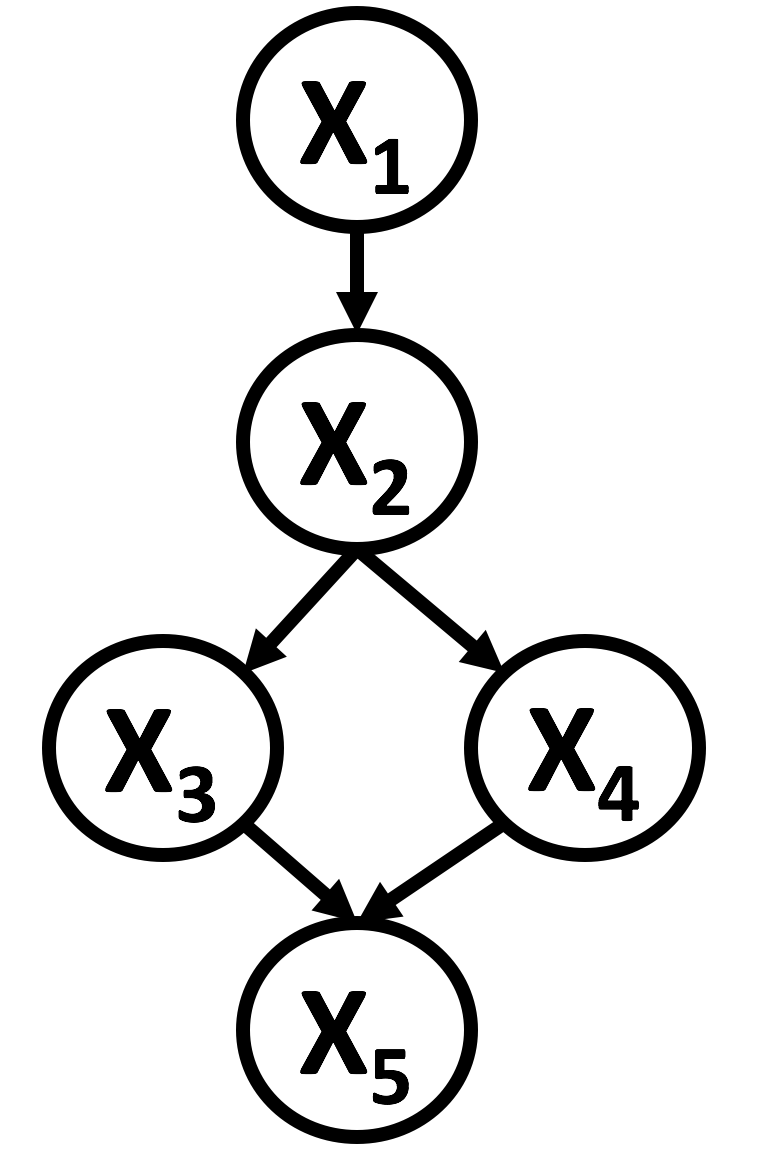
\includegraphics[scale=0.3]{figures/q2.png}
\end{figure}

\begin{enumerate}
\item \textbf{[3pt]} Write down the factorization of the above directed graphical model.

\begin{tcolorbox}[fit,height=1cm, width=15cm, blank, borderline={1pt}{-2pt},nobeforeafter]
%solution
\end{tcolorbox}


\item \textbf{[3pt]} Each random variable represented in the above Bayesian network is binary valued (i.e. either the event happens or it does not). State the minimum number of parameters you need to fully specify  this Bayesian network.

\begin{tcolorbox}[fit,height=1cm, width=2cm, blank, borderline={1pt}{-2pt},nobeforeafter]
%solution
\end{tcolorbox}


\item \textbf{[3pt]} If we didn't use these conditional independence assumptions above, what would be the minimum number of parameters we would need to model any joint distribution over the same set of random variables?

\begin{tcolorbox}[fit,height=1cm, width=2cm, blank, borderline={1pt}{-2pt},nobeforeafter]
%solution
\end{tcolorbox}



\item \textbf{[10pts]} For the following questions fill in the blank with the smallest set $\mathcal{S}$ of random variables needed to be conditioned on in order for the independence assumption to hold. For example $X_i \perp X_j \mid \mathcal{S}$. What is the smallest set $\mathcal{S}$ that makes this statement true? The empty set $\emptyset$ is a valid answer, additionally if the independence assumption cannot be satisfied no matter what we condition on then your answer should be 'Not possible'.
\begin{enumerate}

\item \textbf{[2pt]} $X_1 \perp X_3 \mid $ \begin{tcolorbox}[fit,height=1cm, width=2cm, blank, borderline={1pt}{-2pt},nobeforeafter]
%solution 
\end{tcolorbox}  \\

\item \textbf{[2pt]} $X_1 \perp X_5 \mid$ \begin{tcolorbox}[fit,height=1cm, width=2cm, blank, borderline={1pt}{-2pt},nobeforeafter]
%solution 
\end{tcolorbox}   \\

\item \textbf{[2pt]} $X_2 \perp X_4 \mid $ \begin{tcolorbox}[fit,height=1cm, width=2cm, blank, borderline={1pt}{-2pt},nobeforeafter]
%solution 
\end{tcolorbox}  \\

\item \textbf{[2pt]} $X_3 \perp X_4 \mid $ \begin{tcolorbox}[fit,height=1cm, width=2cm, blank, borderline={1pt}{-2pt},nobeforeafter]
%solution 
\end{tcolorbox}  \\

\item \textbf{[2pt]} $X_2 \perp X_5 \mid $ \begin{tcolorbox}[fit,height=1cm, width=2cm, blank, borderline={1pt}{-2pt},nobeforeafter]
%solution 
\end{tcolorbox}  \\

\end{enumerate}

\clearpage
\item \textbf{[5pts]} Jon gets his friend Sam to calculate some estimates of his chances. Sam returns to Jon with the following conditional probabilities tables:

\begin{table}[H]
    \centering
    \begin{tabular}{|c|c|}
    \hline
         $X_1=0$ & $0.3$  \\ \hline
         $X_1=1$ & $0.7$    \\  \hline
    \end{tabular}
    \\ 
    \begin{tabular}{|c|c|c|}
    \hline
            & $X_1=0$ & $X_1=1$   \\  \hline
        $X_2=0$ & $0.8$ & $0.25$ \\  \hline
        $X_2=1$ & $0.2$  & $0.75$    \\  \hline
    \end{tabular}
    \\ 
    \begin{tabular}{|c|c|c|}
    \hline
            & $X_2=0$ & $X_2=1$   \\  \hline
        $X_3=0$ & $0.5$ & $0.6$ \\  \hline
        $X_3=1$ & $0.5$  & $0.4$    \\  \hline
    \end{tabular}
    \\ 
    \begin{tabular}{|c|c|c|}
    \hline
            & $X_2=0$ & $X_2=1$   \\  \hline
        $X_4=0$ & $0.3$ & $0.2$ \\  \hline
        $X_4=1$ & $0.7$  & $0.8$    \\  \hline
    \end{tabular}
    \\ 
    \begin{tabular}{|c|c|c|c|c|}
    \hline
            & $X_3=0, X_4=0$ & $X_3=0,X_4=1$ & $X_3=1,X_4=0$ & $X_4=1,X_3=1$   \\  \hline
        $X_5=0$ & $0.4$ & $0.7$ & $0.8$ & $0.5$ \\  \hline
        $X_5=1$ & $0.6$  & $0.3$ & $0.2$ & $0.5$    \\  \hline
    \end{tabular}
    \caption{Sam's Conditional Probability tables}
\end{table}

Using the conditional probabilities for our graphical model, compute the following (Your answers should be given to 5 decimal places): 
\begin{enumerate}
\item \textbf{[2pts]} $P(X_1=0, X_2=1, X_3=0, X_4=1, X_5=0)$. 


\begin{tcolorbox}[fit,height=1cm, width=4cm, blank, borderline={1pt}{-2pt},nobeforeafter]
%solution 
\end{tcolorbox}\\


\item \textbf{[3pts]}$P(X_1 = 1 | X_3 = 1)$ 

\begin{tcolorbox}[fit,height=1cm, width=4cm, blank, borderline={1pt}{-2pt},nobeforeafter]
%solution 
\end{tcolorbox}\\

\end{enumerate}
\end{enumerate}

\newpage

\clearpage
\section{Support Vector Machines [14 pts]}

 In class, we discussed the properties and formulation of hard-margin SVMs, where we assume the decision boundary to be linear and attempt to find the hyperplane with the largest margin. Here, we introduce a new class of SVM called soft margin SVM, where we introduce the slack variables $e_i$ to the optimization problem and relax the assumptions. The formulation of soft margin SVM with no Kernel is
    \begin{equation*}
    \begin{aligned}
    & \underset{\mathbf{w}, b, e}{\text{minimize}}
    & & \frac{1}{2}\|\mathbf{w}\|_2^2 + C\left(\sum_{i = 1}^N e_i\right)\\
    & \text{subject to}
    & & y^{(i)}(\mathbf{w}^T\mathbf{x}^{(i)} + b) \geq 1 - e_i, \, \, \forall \; i = 1, \dots, N\\
    & & & e_i \geq 0, \, \, \forall \; i = 1, \dots, N
    \end{aligned}
    \end{equation*}
\begin{enumerate}
    \item \textbf{[3pts]} Consider the $i$th training example $(\mathbf{x}^{(i)}, y^{(i)})$ and its corresponding slack variable $e_i$. Assuming $C > 0$ and is fixed, what would happen as $e_i \rightarrow \infty$?
    
    \textbf{Select all that apply:}
    \begin{list}{}
        \item $\square$ the constraint $y^{(i)}(\mathbf{w}^T\mathbf{x}^{(i)} + b) \geq 1 - e_i$ would hold for any $\mathbf{w}$ with finite entries.
        \item $\square$ there would be no vector that satisfies the constraint $y^{(i)}(\mathbf{w}^T\mathbf{x}^{(i)} + b) \geq 1 - e_i$
        \item $\square$ the objective function would approach infinity.
    \end{list}
    
    
    With this in mind, we hope that you can see why soft margin SVM can be applied even when the data is not linearly separable.
    
    
    %\clearpage
    
    % Adjusting C in soft margin SVMs
    \item \textbf{[4pts]} Which of the following are true when $C \rightarrow \infty$? Assume that the data is \textbf{not} linearly separable, unless otherwise specified.
    
    \textbf{Select all that apply:}
    
        \begin{list}{}
        \item $\square$ When the data is linearly separable, the solution to the soft margin SVM would converge to the solution of hard margin SVM.
        \item $\square$ There is no solution $\mathbf{w}, b$ satisfying all the constraints in the optimization problem with a non-infinite objective value.
        % CONFUSING: \item $\square$ Any arbitrary vector $\mathbf{w}$ and scalar $b$ can satisfy the constraints in the optimization problem.
        \item $\square$ The optimal weight vector would converge to the zero vector $\mathbf{0}$.
        \item $\square$ When $C$ approaches to infinity, it could help reduce overfitting.
    \end{list}
    
    
    \clearpage
    
    \item \textbf{[4pts]} Which of the following are true when $C \rightarrow 0$? Assume that the data is \textbf{not} linearly separable, unless otherwise specified.
    
    \textbf{Select all that apply:}
    
    \begin{list}{}
        \item $\square$ When the data is linearly separable, the solution to the soft margin SVM would converge to the solution of hard margin SVM.
        \item $\square$ There is no solution $\mathbf{w}, b$ satisfying all the constraints in the optimization problem with a non-infinite objective value.
        % CONFUSING: \item $\square$ Any arbitrary vector $\mathbf{w}$ and scalar $b$ can satisfy the constraints in the optimization problem.
        \item $\square$ The optimal weight vector would converge to be the zero vector $\mathbf{0}$.
        \item $\square$ When $C$ approaches to 0, doing so could help reduce overfitting.
    \end{list}
    
    %\clearpage
    
    \item \textbf{[3pts]} An extension to soft margin SVM (or, an extension to the hard margin SVM we talked in class) is the 2-norm SVM with the following primal formulation
    
    \begin{equation*}
        \begin{aligned}
        & \underset{\mathbf{w}, b, e}{\text{minimize}}
        & & \frac{1}{2}\|\mathbf{w}\|_2^2 + C\left(\sum_{i = 1}^N e_i^2\right)\\
        & \text{subject to}
        & & y^{(i)}(\mathbf{w}^T\mathbf{x}^{(i)} + b) \geq 1 - e_i, \, \, \forall \; i = 1, \dots, N\\
        & & & e_i \geq 0, \, \, \forall \; i = 1, \dots N
        \end{aligned}
    \end{equation*}
    
    Which of the following is true about the 2-norm SVM? (Hint: think about $\ell_1$-regularization versus $\ell_2$ regularization!)
    
    \textbf{Select one:}
        \begin{list}{}
        \item $\circle$ If a particular pair of parameters $\mathbf{w}^*, b^*$ minimizes the objective function in soft margin SVM, then this pair of parameters is guaranteed to minimize the objective function in 2-norm SVM.
        \item $\circle$ 2-norm SVM penalizes large $e_i$'s more heavily than soft margin SVM.
        \item $\circle$ One drawback of 2-norm SVM is that it cannot utilize the kernel trick.
        \item $\circle$ None of the above.
    \end{list}
    
    
    % \begin{figure}[H]
    %   \centering
    %      \includegraphics[width=0.7\linewidth]{figures/svm}
    %      \caption{SVM dataset}
    %   \label{fig:SVM}
    %  \end{figure}
    % \item \textbf{[3pts]} Consider the dataset shown in Figure~\ref{fig:SVM}. Which of the following models, when properly tuned, could correctly classify \textbf{ALL} the data points?
    
    % \textbf{Select all that apply:}
    
    %     \begin{list}{}
    % \item $\square$ Logistic Regression without any kernel
    % \item $\square$ Hard margin SVM without any kernel
    % \item $\square$ Soft margin SVM without any kernel
    % \item $\square$ Hard margin SVM with RBF Kernel
    % \item $\square$ Soft margin SVM with RBF Kernel
    % \end{list}
    
    \end{enumerate}
    
    \clearpage
    \begin{comment}
    \section{Kernels [19pts]}
    \begin{enumerate}
    \item \textbf{[2pt]} Consider the following kernel function:

    \[K(\xv, \xv') = \begin{cases}{\text{1,  if } \xv = \xv'} \\{\text{0,  otherwise}}\end{cases}\]

    \textbf{True or False:} In this kernel space, any labeling of a set of instances $\{\xv^{(1)}, \xv^{(2)}, \ldots, \xv^{(N)} \}$ from a training set will be linearly separable. Assume that no two points in this instance set are identical.

    \begin{list}{}
        \item $\circle$ True
        \item $\circle$ False
    \end{list}
    
    
    \item \textbf{[3pts]} Suppose that input-space is two-dimensional, \( x = (x_1, x_2)^T\). The feature mapping is defined as - \[\phi(x) = (x_1^2, x_2^2, 1, \sqrt{2}x_1x_2, \sqrt{2}x_1,\sqrt{2}x_2)^T\]
    
    What is the corresponding kernel function, i.e. \(K(x,z)\)? \textbf{Select one.}

    
    \begin{list}{}
        \item $\circle$ \( (x_1z_1)^2 +(x_2z_2)^2 +1 \)
        \item $\circle$ \( (1 + x^T z)^2 \)
        \item $\circle$ \( (x^T z)^2 \)
        \item $\circle$ \( x^T z \)
    \end{list}
    
    \item \textbf{[3pts]} Suppose that input-space is three-dimensional, \( x = (x_1, x_2, x_3)^T\). The feature mapping is defined as - \[\phi(x) = (x_1^2, x_2^2, x_3^2, \sqrt{2}x_1x_2, \sqrt{2}x_1x_3,\sqrt{2}x_2x_3)^T\]

    Suppose we want to compute the value of kernel function \(K(x,z)\) on two vectors \(x,z \in {\mathbb{R}}^3\). We want to check how many additions and multiplications are needed if you map the input vector to the feature space and then perform dot product on the mapped features. Report \(\alpha + \beta\), where \(\alpha\) is the number of multiplications and \(\beta\) is the number of additions.

    Note: Multiplication/Addition with constants should also be included in the counts.
    
    \begin{tcolorbox}[fit,height=1cm, width=2cm, blank, borderline={1pt}{-2pt},nobeforeafter]
    %solution
    \end{tcolorbox}
    
    \item \textbf{[3pts]} Suppose that input-space is three-dimensional, \( x = (x_1, x_2, x_3)^T\). The feature mapping is defined as - \[\phi(x) = (x_1^2, x_2^2, x_3^2, \sqrt{2}x_1x_2, \sqrt{2}x_1x_3,\sqrt{2}x_2x_3)^T\]

    Suppose we want to compute the value of kernel function \(K(x,z)\) on two vectors \(x,z \in {\mathbb{R}}^3\).We want to check how many additions and multiplications are needed if you do the computation through the kernel function you derived above. Report \(\alpha + \beta\), where \(\alpha\) is the number of multiplications and \(\beta\) is the number of additions.

    Note: Multiplication/Addition with constants should also be included in the counts.
    
    \begin{tcolorbox}[fit,height=1cm, width=2cm, blank, borderline={1pt}{-2pt},nobeforeafter]
    %solution
    \end{tcolorbox}
    
    
    \item \textbf{[3pts]} Suppose one dataset contains four data points in \(\R^1\) space, as shown in Figure~\ref{fig:lindata}

    \begin{figure}[H]
    \centering
        \includegraphics[width=0.7\linewidth]{figures/lineardataset.png}
        \caption{Data in $\R^1$}
        \label{fig:lindata}
    \end{figure}


    Different shapes of the points indicate different labels. If we train a linear classifier on the dataset, what is the lowest training error for a linear classifier on \(\R^1\)?
    
    \begin{tcolorbox}[fit,height=1cm, width=2cm, blank, borderline={1pt}{-2pt},nobeforeafter]
    %solution
    \end{tcolorbox}
    
    \item \textbf{[3pts]} Following the above question, which of the feature mappings below can we use to project the dataset to higher dimensional space such that training a linear classifier on the projected dataset would yield zero training error?
        \begin{list}{}
        \item $\circle$ \(\phi(x) = (x, 1)\)
        \item $\circle$ \(\phi(x) = (x, x^3)\)
        \item $\circle$ \(\phi(x) = (x, x^2)\)
        \item $\circle$ \(\phi(x) = (x, (x+1)^2)\)
    \end{list}

    
    
    \item \textbf{[2pt]} \textbf{True or False:} Given the same training data, in which the points are linearly separable, the margin of the decision boundary produced by SVM will always be greater than or equal to the margin of the decision boundary produced by Perceptron.
    
    \begin{list}{}
        \item $\circle$ True
        \item $\circle$ False
    \end{list}
    
    
\end{enumerate}
\clearpage
% \section{EM}
% \begin{center}
%     \textbf{!!!Listed in Slack channel as a potential topic but was not discussed in lecture! Included for completeness!!!}
% \end{center}
% \begin{enumerate}
%     \item Which of the following is \textbf{correct} about EM?
    
%     \textbf{Select one:}
%     \begin{list}{}
%         \item $\circle$ The EM algorithm is guaranteed to converge to the global optimum.
%         \item $\circle$ If we start the EM algorithm with different starting values, we are guaranteed to obtain the same solution after the algorithm converges.
%         \item $\circle$ It is possible for the objective function to decrease during an iteration of EM.
%         \item $\circle$ None of the above.
%     \end{list}
    
% \end{enumerate}
%\clearpage
\end{comment}
\clearpage
\section{PCA [11pts]}

\begin{enumerate}
    \item \textbf{[3pts]} Assume we are given a dataset X for which the eigenvalues of the covariance matrix are:
    (2.2, 1.7, 1.4, 0.8, 0.4, 0.2, 0.15, 0.02, 0.001). What is the smallest value of k we can use if we want to retain 75\% of the variance (sum of all the variances in value) using the first k principal components?
    
    \begin{tcolorbox}[fit,height=1cm, width=2cm, blank, borderline={1pt}{-2pt},nobeforeafter]
    %solution
    \end{tcolorbox}
    
    
    \item \textbf{[2pts]} Assume we apply PCA to a matrix $X \in R^{n \times m}$ and obtain a set of PCA features, $Z \in R^{n \times m}$ .We divide this set into two, $Z1$ and $Z2$.The first set, Z1, corresponds to the top principal components. The second set, Z2, corresponds to the remaining principal components. Which is more common in the training data:
    \textbf{Select one:}
    \begin{list}{}
        \item $\circle$ a point with large feature values in $Z1$ and small feature values in  $Z2$
        \item $\circle$ a point with large feature values in $Z2$ and small feature values in  $Z1$
        \item $\circle$ a point with large feature values in $Z2$ and large feature values in  $Z1$
        \item $\circle$ a point with small feature values in $Z2$ and small feature values in  $Z1$
    \end{list}
    
\clearpage    
Use the figure below to answer the following questions.    
    \begin{figure}[H]
    \centering
    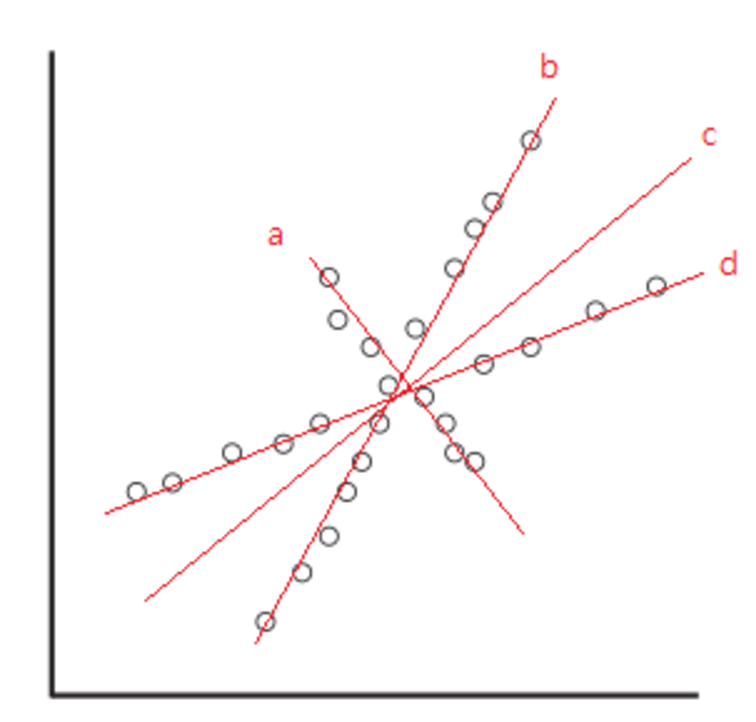
\includegraphics[width=0.5\linewidth]{figures/pca1.png}
    \end{figure}
    
\item \textbf{[2pts]} What will be its first principal component? %Options are given in the form of (first Principal Component, second Principal Component).
    \textbf{Select one:}
    \begin{list}{}
        %\item $\circle$ (a,b)
        \item $\circle$ d %(d,b)
        \item $\circle$ b %(b,d)
        \item $\circle$ c %(c,a)
        \item $\circle$ a %(a,c)
        
    \end{list}
    
    \item \textbf{[2pts]} \textbf{NOTE : This is continued from the previous question.} What is the second principal component in the figure from the previous question? %Options are given in the form of (first Principal Component, second Principal Component).
    % \begin{figure}[H]
    % \centering
    % 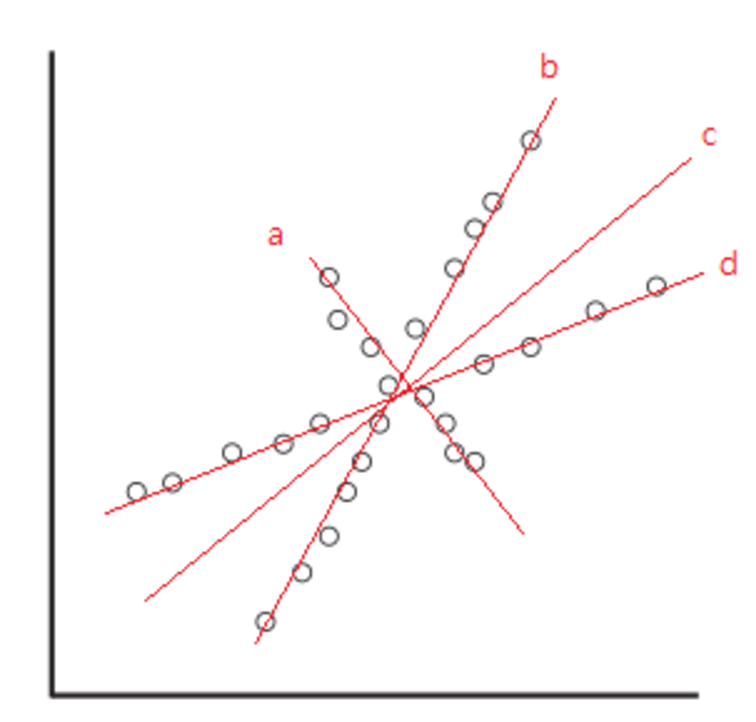
\includegraphics[width=0.65\linewidth]{figures/pca1.png}
    % \end{figure}
    \textbf{Select one:}
    \begin{list}{}
        %\item $\circle$ (a,b)
        \item $\circle$ d %(d,b)
        \item $\circle$ b %(b,d)
        \item $\circle$ c %(c,a)
        \item $\circle$ a %(a,c)
        
    \end{list}
    \item \textbf{[2pts]} \textbf{NOTE : This is continued from the previous question.}
What is the third principal component in the figure from the previous question?
     \textbf{Select one:}
    \begin{list}{}
        \item $\circle$ a
        \item $\circle$ b
        \item $\circle$ c
        \item $\circle$ d
        \item $\circle$ None of the above
        
    \end{list}

\end{enumerate}
\clearpage
\clearpage





\begin{comment} 
{\bf Collaboration Questions} After you have completed all other components of this assignment, report your answers to the collaboration policy questions detailed in the Academic Integrity Policies found \href{http://www.cs.cmu.edu/~mgormley/courses/10601-s18/about.html#7-academic-integrity-policies}{here}.
    \begin{enumerate*}
        \item Did you receive any help whatsoever from anyone in solving this assignment? If so, include full details.
        \item Did you give any help whatsoever to anyone in solving this assignment? If so, include full details?
        \item Did you find or come across code that implements any part of this assignment ? If so, include full details.
    \end{enumerate*}
    
    \begin{tcolorbox}[fit,height=3cm,blank, borderline={1pt}{-2pt},nobeforeafter]
    %Input your solution here.  Do not change any of the specifications of this solution box.
    \end{tcolorbox}
\end{comment}


\textbf{Collaboration Questions} Please answer the following:


    After you have completed all other components of this assignment, report your answers to the collaboration policy questions detailed in the Academic Integrity Policies found \href{http://www.cs.cmu.edu/~mgormley/courses/10601bd-f18/about.html#7-academic-integrity-policies}{here}.
    \begin{enumerate}
        \item Did you receive any help whatsoever from anyone in solving this assignment? Is so, include full details.
        \item Did you give any help whatsoever to anyone in solving this assignment? Is so, include full details.
        \item Did you find or come across code that implements any part of this assignment ? If so, include full details.
    \end{enumerate}
    
    \begin{solution}
    % If you are using the latex template, remove the empty spaces
    \bigskip \bigskip \bigskip \bigskip \bigskip \bigskip \bigskip \bigskip
    \bigskip \bigskip \bigskip \bigskip \bigskip \bigskip \bigskip \bigskip
    \bigskip \bigskip \bigskip \bigskip \bigskip \bigskip \bigskip \bigskip
    \bigskip \bigskip \bigskip \bigskip \bigskip \bigskip \bigskip \bigskip
    \bigskip \bigskip \bigskip \bigskip \bigskip \bigskip \bigskip \bigskip
    \bigskip \bigskip \bigskip \bigskip \bigskip \bigskip \bigskip \bigskip
    \bigskip \bigskip \bigskip \bigskip \bigskip \bigskip \bigskip \bigskip
    \end{solution}
    

\end{document}
